\documentclass[12pt,a4paper]{article}

% Packages
\usepackage{amsmath}
\usepackage{amssymb}
\usepackage{amsthm}
\usepackage[margin=1in]{geometry}
\usepackage{enumitem}
\usepackage{tikz}
\usepackage{pgfplots}
\pgfplotsset{compat=1.18}

% Custom environments
\newtheorem{explanation}{Explanation}
\theoremstyle{definition}
\newtheorem{solution}{Solution}

% Title information
\title{Methods of Applied Mathematics - Part 1\\
Exercise Sheet 3: Bifurcations - Question 1}
\author{}
\date{}

\begin{document}

\maketitle

\section{Question 1: $\dot{x} = (5-x)(1-ax)$ with $a > 0$}

\begin{solution}

	\textbf{Goal: Find equilibria, their stability, identify the bifurcation at $a = 1/5$, and sketch the bifurcation diagram}

	\vspace{10pt}

	\hrule

	\vspace{10pt}

	\subsection*{Finding Equilibria}

	\textbf{Step 1: Set $\dot{x} = 0$}

	$$(5-x)(1-ax) = 0$$

	\textbf{Step 2: Solve}

	Two equilibria:
	$$\boxed{x_1^* = 5} \quad \text{and} \quad \boxed{x_2^* = \frac{1}{a}}$$

	Note: $x_1^* = 5$ is independent of $a$ (fixed), while $x_2^* = 1/a$ moves as $a$ varies. At $a = 1/5$, both equal 5.

	\vspace{10pt}

	\hrule

	\vspace{10pt}

	\subsection*{Stability Analysis}

	\textbf{Step 1: Compute $f'(x)$ where $f(x) = (5-x)(1-ax)$}

	Expand: $f(x) = 5 - 5ax - x + ax^2$

	Derivative:
	$$f'(x) = -5a - 1 + 2ax$$

	\textbf{Step 2: Evaluate at $x_1^* = 5$}

	$$f'(5) = -5a - 1 + 2a(5) = -5a - 1 + 10a = -1 + 5a$$

	Stability:
	\begin{itemize}
		\item $a < 1/5$: $f'(5) < 0$ $\Rightarrow$ Stable
		\item $a = 1/5$: $f'(5) = 0$ $\Rightarrow$ Neutral
		\item $a > 1/5$: $f'(5) > 0$ $\Rightarrow$ Unstable
	\end{itemize}

	\textbf{Step 3: Evaluate at $x_2^* = 1/a$}

	$$f'(1/a) = -5a - 1 + 2a(1/a) = -5a - 1 + 2 = 1 - 5a$$

	Stability:
	\begin{itemize}
		\item $a < 1/5$: $f'(1/a) > 0$ $\Rightarrow$ Unstable
		\item $a = 1/5$: $f'(1/a) = 0$ $\Rightarrow$ Neutral
		\item $a > 1/5$: $f'(1/a) < 0$ $\Rightarrow$ Stable
	\end{itemize}

	\textbf{Step 4: Summary}

	\begin{center}
		\begin{tabular}{|c|c|c|}
			\hline
			Parameter & $x^* = 5$ & $x^* = 1/a$ \\
			\hline
			$a < 1/5$ & Stable & Unstable \\
			$a = 1/5$ & \multicolumn{2}{c|}{Both at $x=5$, neutral} \\
			$a > 1/5$ & Unstable & Stable \\
			\hline
		\end{tabular}
	\end{center}

	The equilibria exchange stability as they pass through each other at $a = 1/5$.

	\vspace{10pt}

	\hrule

	\vspace{10pt}

	\subsection*{Bifurcation Identification}

	\textbf{Step 1: Check Bifurcation Conditions at $a = 1/5$, $x = 5$}

	(B1) Equilibrium: $f(5) = 0$ \checkmark

	(B2) Zero eigenvalue: $f'(5) = -1 + 5(1/5) = 0$ \checkmark

	(B3) $\partial f/\partial a = -(5-x) \cdot x|_{x=5} = 0$ \checkmark

	\textbf{Step 2: Check Genericity Conditions}

	(G1) $f''(x) = 2a|_{a=1/5} = 2/5 \neq 0$ \checkmark

	(G2) $\partial f'/\partial a = -5 + 2x|_{x=5} = 5 \neq 0$ \checkmark

	\textbf{Conclusion:}
	$$\boxed{\text{Transcritical bifurcation at } a = 1/5}$$

	One equilibrium is pinned at $x=5$, the other passes through it, and they exchange stability.

	\vspace{10pt}

	\hrule

	\vspace{10pt}

	\subsection*{Bifurcation Diagram}

	\textbf{Step 1: Identify branches}

	\begin{itemize}
		\item Branch 1: $x = 5$ (horizontal line)
		      \begin{itemize}
			      \item Stable for $a < 1/5$ (solid)
			      \item Unstable for $a > 1/5$ (dashed)
		      \end{itemize}
		\item Branch 2: $x = 1/a$ (hyperbola)
		      \begin{itemize}
			      \item Unstable for $a < 1/5$ (dashed)
			      \item Stable for $a > 1/5$ (solid)
		      \end{itemize}
	\end{itemize}

	Bifurcation point: $(a, x) = (1/5, 5)$

	\textbf{Step 2: Sketch}

	\begin{center}
		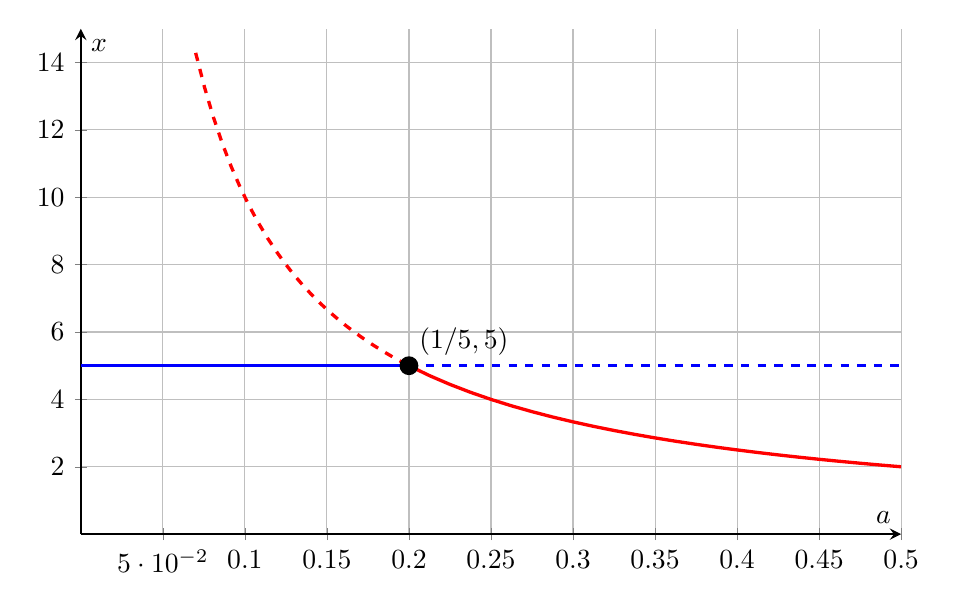
\begin{tikzpicture}
			\begin{axis}[
					width=12cm,
					height=8cm,
					xlabel={$a$},
					ylabel={$x$},
					xmin=0, xmax=0.5,
					ymin=0, ymax=15,
					grid=major,
					axis lines=middle,
					thick
				]

				% x = 5 stable
				\addplot[blue, very thick, solid, domain=0:0.2] {5};

				% x = 5 unstable
				\addplot[blue, very thick, dashed, domain=0.2:0.5] {5};

				% x = 1/a unstable
				\addplot[red, very thick, dashed, domain=0.07:0.2] {1/x};

				% x = 1/a stable
				\addplot[red, very thick, solid, domain=0.2:0.5] {1/x};

				% Bifurcation point
				\addplot[mark=*, mark size=3pt, black] coordinates {(0.2, 5)};
				\node[above right] at (axis cs:0.2,5) {$(1/5, 5)$};

			\end{axis}
		\end{tikzpicture}
	\end{center}

	Solid = stable, dashed = unstable

	\vspace{10pt}

	\hrule

	\vspace{10pt}

	\subsection*{Summary}

	\begin{itemize}
		\item Equilibria: $x^* = 5$ and $x^* = 1/a$
		\item At $a = 1/5$: transcritical bifurcation where equilibria collide and exchange stability
		\item For $a < 1/5$: $x=5$ stable, $x=1/a$ unstable
		\item For $a > 1/5$: $x=5$ unstable, $x=1/a$ stable
	\end{itemize}

\end{solution}

\end{document}
